\documentclass[a4paper,11pt]{article}

\usepackage{graphicx}
\usepackage{subfig,hyperref}
\newcommand{\HRule}{\rule{\linewidth}{0.5mm}}

\begin{document}
\pagenumbering{alph}
\begin{titlepage}
\begin{center}

\textsc{\LARGE CMSC726 Machine Learning}\\[1.5cm]

\textsc{\Large Project 2}\\[0.5cm]

\HRule \\[0.5cm]

{ \huge \bfseries Complex Classification}\\[0.4cm]

\HRule \\[1.5cm]

{\large Angjoo Kanazawa, Ran Liu, and Austin Myers}

\vfill

{\large November 1, 2011}

\end{center}
\end{titlepage}
%\title{ML CS726 Fall'11 Project 2 Complex Classifiers}
%\author{Angjoo Kanazawa, Ran Liu, Austin Myers}
%\maketitle
\pagenumbering{arabic}

\section{Gradient Descent and Linear Classification}
\subsection{WU1}
\textsf{Find a few values of step size where it converges and a few
  values where it diverges. Where does the threshold seem to be?}\\

It depends on what the number of iteration is, but with 100
iterations, from step 0.1 to 6.5 it finds a solution close to
0. But right after 6.6, it starts to diverge and for any value after
6.7 it diverges, so the threshold seems to be around 6.6.

\subsection{WU2}
\textsf{Come up with a non-convex univariate optimization
  problem. Plot the function you're trying to minimize and show two
  runs of gd, one where it gets caught in a local minimum and one
  where it manages to make it to a global minimum. (Use different
  starting points to accomplish this.)}\\

Using $f(x) = sin(\pi x) + x^2/2$, $f'(x) = \pi cos(\pi x) + x$, and
10 iterations, the
global minimum happens at $x\approx -0.45385$.
If we start at 0, we can find the global minimum, but if we start at
1, gd gets caught in a local minimum $1.357$

Output:
\begin{verbatim}
>>> gd.gd(f, derF, 0, 10, 0.2)
(-0.45385351939658519, array([ 0 -0.72244765, 
 -0.84494752, -0.88472033, -0.88650671, 
 -0.88651822, -0.88651823, -0.88651823, 
 -0.88651823, -0.88651823, -0.88651823]))
>>> gd.gd(f, derF, 1, 10, 0.2)
(1.3577434052579487, 
 array([  1.22464680e-16, 4.52961014e-02,
 2.50055080e-02, 2.00175811e-02, 1.99477186e-02, 
 1.99477147e-02, 1.99477147e-02, 1.99477147e-02, 
 1.99477147e-02, 1.99477147e-02, 1.99477147e-02]))
\end{verbatim}

The first run finds the global minimum, but the second one
doesn't (the first value in the ouptut of gd is the solution it found).

\subsection{WU3 - Not Required}
%\textsf{Why does the logistic classifier produce much larger weights
%  than the others, even though they all get basically the same
%  classification performance?}\\ Don't have to answer this.

\newpage

\begin{figure}[!ht]
  \begin{center}
  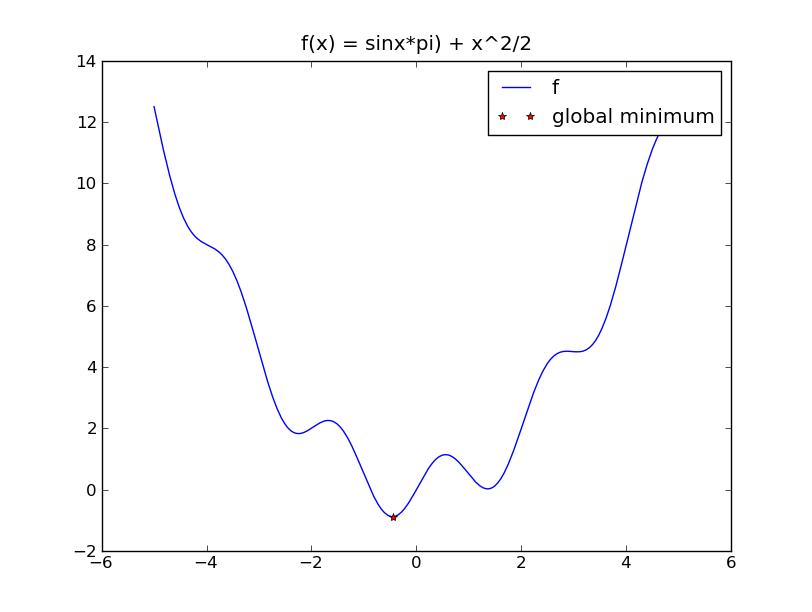
\includegraphics[width=5in]{wu2.png}
  \caption{WU2: $f(x) = sin(\pi x) + x^2/2$, $f'(x) = \pi cos(\pi x) + x$}
  \end{center}
\end{figure}

\newpage

\section{Warm Up with ML Tools}
\label{sec:warmup}
\subsection{WU4}
\textsf{What are the five features with largest positive weight and what
are the five features with largest negative weight? Do these seem "right"
based on the task?}\\

The features with the largest positive and negative weights are shown in 
Table \ref{tables:WU4Pos} and Table \ref{tables:WU4Neg} respectively. 
Some features, like the ``xx'' feature, do not seem to have a understandable 
meaning. However, many features do seem "right" according to their field.
The features corresponding to graphics documents include ``graphics'', 
``image(s)'', and ``card'' which all are easily related to the topic. 
The features associated with windows include ``motif'', ``window'', and ``x''
which makes sense since Motif is a GUI widget toolkit under the X Window System. 
Therefore, it appears that the largest weights have some understandable meanings.

\begin{table}[!ht]
\begin{center}
    \begin{tabular}{| l | l |}
    \hline
    Feature  & Weight \\ \hline
    graphics & 1.0918 \\ \hline %Raw 1.09135174751281738281
    images   & 0.7224 \\ \hline %Raw 0.72243607044219970703
    image    & 0.7200 \\ \hline %Raw 0.72001230716705322266
    card     & 0.7124 \\ \hline %Raw 0.71239823102951049805
    xx       & 0.6912 \\ \hline %Raw 0.69124054908752441406
    \end{tabular}
    \caption{The five features with the largest positive weights.}
    \label{tables:WU4Pos}
\end{center}
\end{table}

\begin{table}[!ht]
\begin{center}
    \begin{tabular}{| l | l |}
    \hline
    Feature &  Weight \\ \hline
    motif   & -1.2143 \\ \hline %Raw -1.21427941322326660156
    window  & -1.1542 \\ \hline %Raw -1.15418136119842529297
    server  & -0.9483 \\ \hline %Raw -0.94833439588546752930
    list    & -0.8908 \\ \hline %Raw -0.89077484607696533203
    x       & -0.8657 \\ \hline %Raw -0.86568439006805419922
    \end{tabular}
    \caption{The five features with the largest negative weights.}
    \label{tables:WU4Neg}
\end{center}
\end{table}

\newpage

\subsection{WU5}
\textsf{Draw the tree. How do the selected features compare to the
  features from the logistic regression model? Which features seem
  "better" and why? If you use a depth 10 tree, how well do you do on
  test data?}\\

\begin{figure}[!ht]
  \begin{center}
  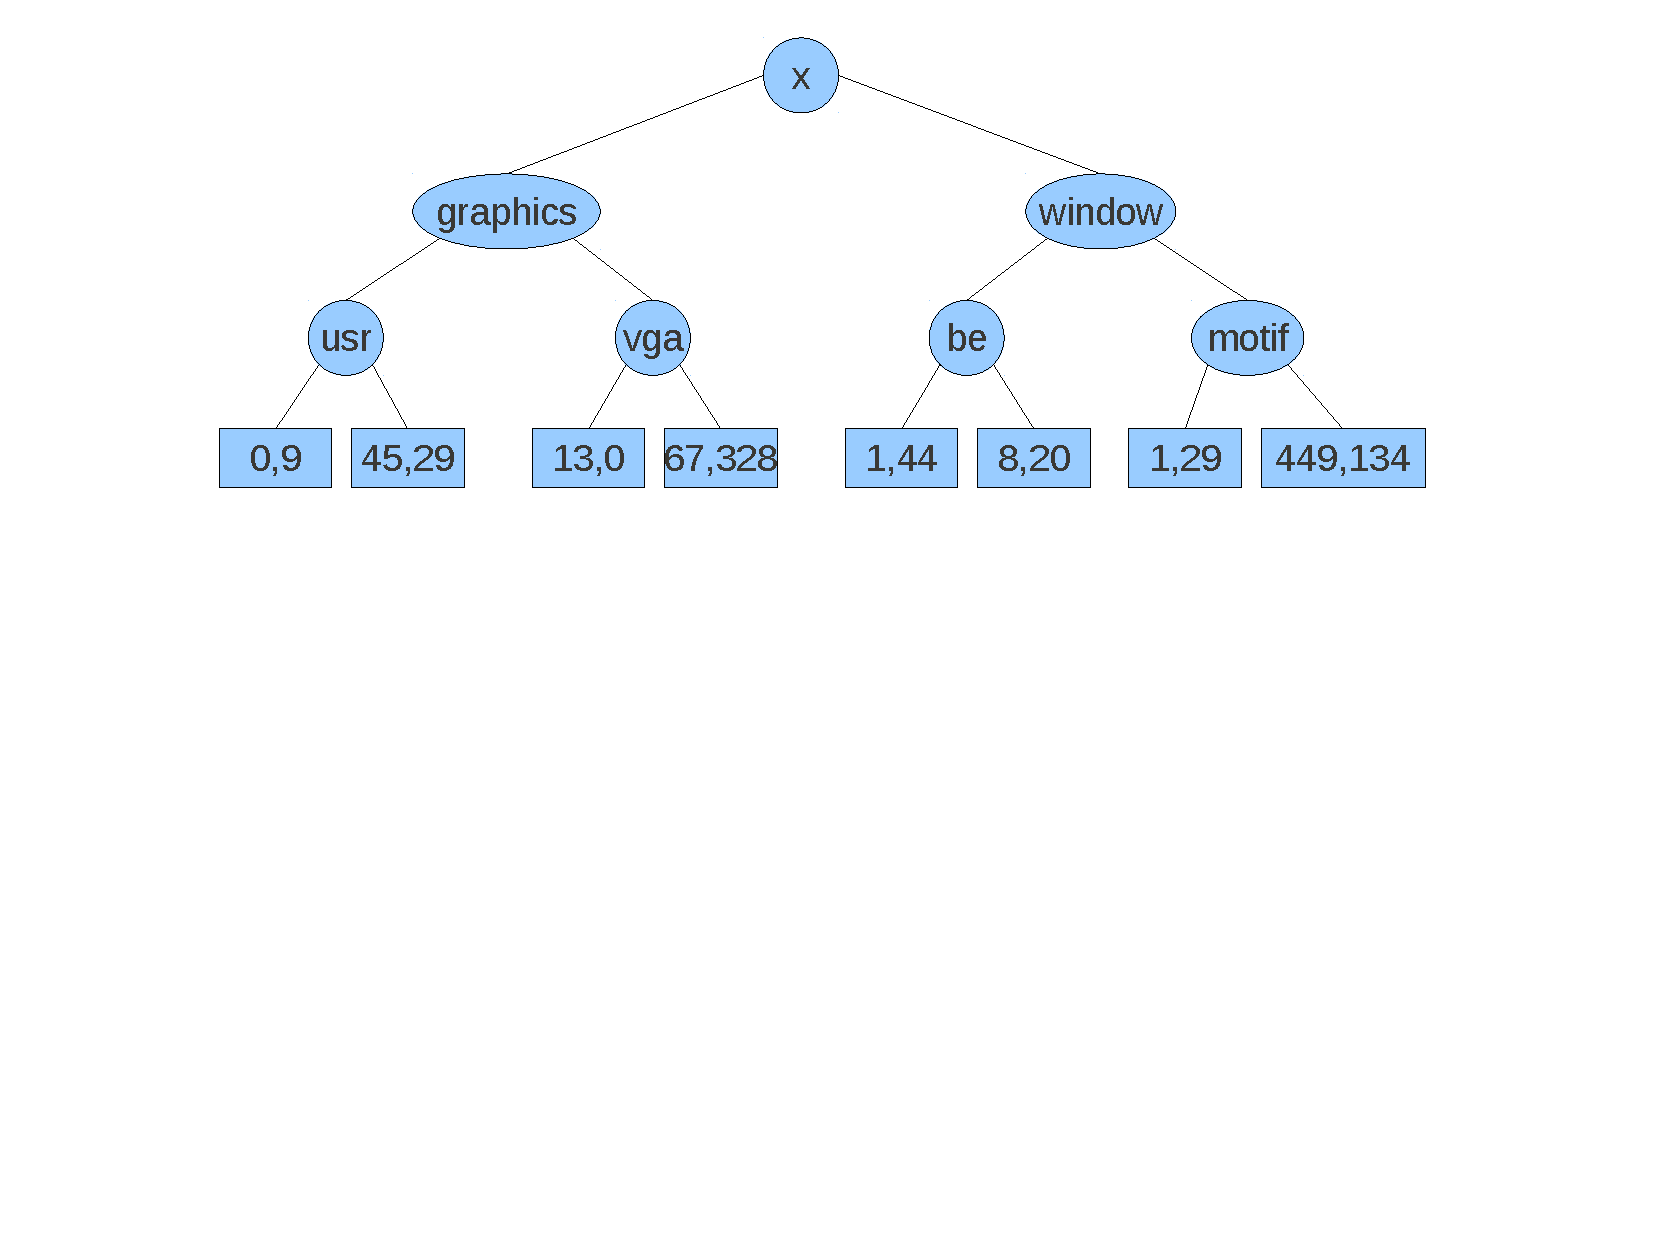
\includegraphics[width=4.75in]{wu5_tree.pdf}
  \caption{WU5: The tree}
  \end{center}
\end{figure}

Features can be considered ``better'' if they are decisive, 
when the ratio bewteen class 1 and class -1 at the leaf is high, 
and if they are robust, when many instances have corroborate the decision.

The features selected by the FastDT algorithm agree with four of the most
positive and negative weighted features from the Megam algorithm; these 
include ``graphics'', ``motif'', ``window'', and ``x''. In detail, 
``motif'' and ``vga'' are the better features. ``motif'' has high frequency
(total 583 instances fall have no motif) and high ratio (about 80\% of
those without ``motif'' are in class 1). For ``vga``,  395 instances fall into
the class 1, and 84\% of those with no ``vga'' are in class -1. If they
have ``vga'', 100\% of them are in class 1. However, this may not be the
most reliable indicator because only 13 data falls into yes ``vga''.
In this respect, ``usr'' is one of the least useful of the features selected
for the tree because the relative frequency is low, and when there is no ``usr'',
the ratio of class 1 to class -1 is 6:4.

The depth of the decision tree can be increased to increase the potential number
of decisions. If the depth of the tree is increased to 10 levels for this task,
the test error is reduced by 0.463\% to 20.53\%. This implies that the nodes at higher
levels in the tree are mostly sufficient for the classification task, and increasing
depth beyond this point does not yield a significant boost in accuracy.

\subsection{WU6}
\textsf{Using comp.graphics versus comp.windows.x, plot training 
and test error curves for each of the algorithms. 
For megam, use lambda values of $2^x, -5 \leq x \leq 5$. 
For FastDT, use depths 1 through 20. 
For libsvm, use C values of $2^x,  -5 \leq x \leq 5$. 
Before actually running these experiments, what do you expect to happen? 
What actually does happen?}\\

\begin{figure}[!ht]
  \begin{center}
  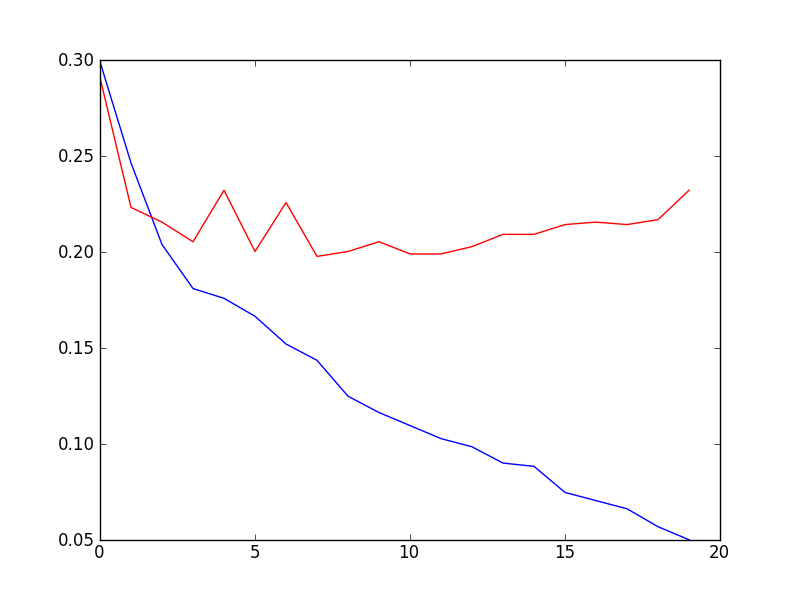
\includegraphics[width=4.5in]{WU6/learningCurve_FastDT.png}
  \label{figures:wu61}
  \end{center}
\end{figure}
\begin{figure}[!ht]
  \begin{center}
  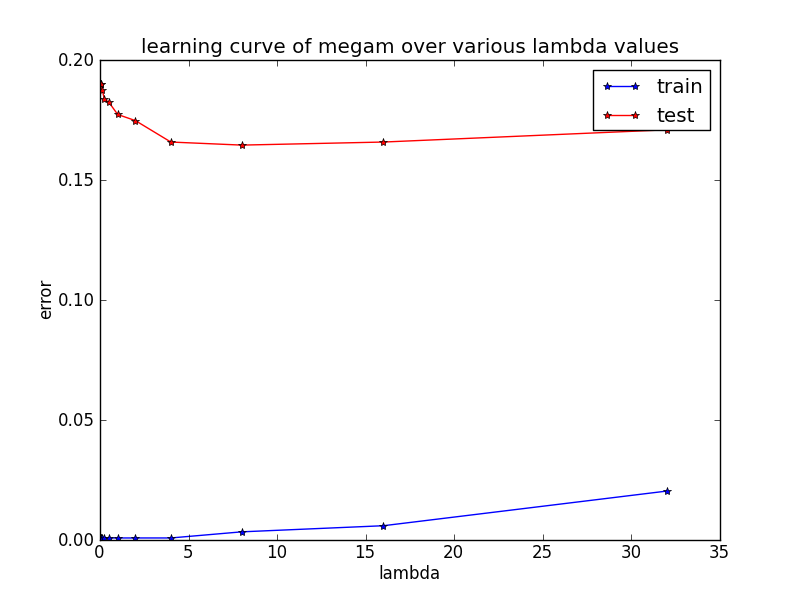
\includegraphics[width=4.5in]{WU6/learningCurve_megam.png}
    \label{figures:wu62}
  \end{center}
\end{figure}
\begin{figure}[!ht]
  \begin{center}
  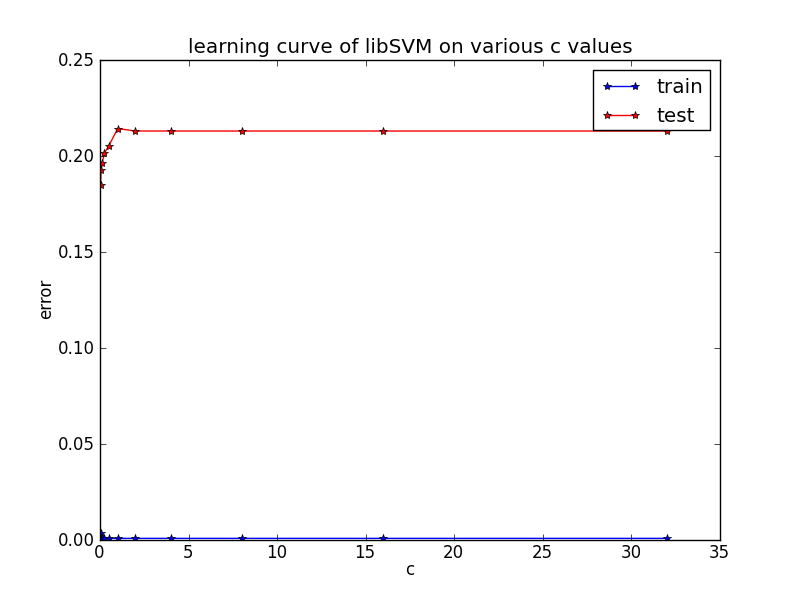
\includegraphics[width=4.5in]{WU6/learningCurve_libsvm.png}
    \label{figures:wu63}
  \end{center}
\end{figure}

Figure \ref{figures:wu61}shows the learning curve for FastDT, where the blue curve is the the training error and red curve is the test error. I expected the training error reduce to a really small number with the increasing of the depth of the tree. The testing error will go down at the beginning and will go up later because of the overfitting. As shown in the figure, the plot is similar to what i expected.

Figure  \ref{figures:wu62} shows the learning curve for Megam. The expected training error is to be smaller and smaller but in this plot, the training error goes up. 

Figure \ref{figures:wu63}shows the learning curve for libsvm.  I expected the training error reduce to a really small number with the increasing of the depth of the tree. The testing error will go down at the beginning and will go up later because of the overfitting. As shown in the figure, the plot is similar to what i expected.


\subsection{WU7}
\textsf{Comparing the performance of the three different algorithms 
on the two tasks (text categorization versus digit recognition), 
which one(s) perform best on one and which on the other? Why?}\\

The performances of each algorithm on the text and digit classification 
tasks are shown in Table \ref{tables:WU7}. We see that for text 
classification FastDT and libSVM perform similarly, while Megam achieves a 
few extra percentage points for accuracy. For digit classification Megam and 
libSVM perform identically, and with higher accuracy than FastDT. One 
explanation for this difference would be that the text classification data 
can be separated linearly using a few basic features so all algorithms 
perform similarly, but this approach to digit classification uses very fine 
grained pixel level features which are not as useful for the decision tree 
model. If we used high level image features, like histograms, SIFT, or 
wavelets, we might find that the decision tree would be on par with
its competitors.

\begin{table}[!ht]
\begin{center}
    \begin{tabular}{ | l | l | l |} \hline
    Algorithm & Text   & Digit \\ \hline
    Megam     & 82.3\% & 93.0\% \\ \hline
    FastDT    & 79.5\% & 88.0\% \\ \hline
    libSVM    & 78.5\% & 93.0\% \\ \hline
    \end{tabular}
    \caption{Accuracy of Algorithms for Text and Digit Classification}
    \label{tables:WU7}
\end{center}
\end{table}

\pagebreak
\section{Reductions for Multiclass Classification}
\subsection{WU8}
\textsf{For each of the three reductions, run your classifier on the
text classification problem with four classes. For the tree reduction, 
make the first split {graphics,windows} versus {baseball,hockey}. 
Tune your hyperparameters as well as you can and report the best 
results you can for each of the three. Which one wins? Which one was 
easiest to tune hyperparameters for?}\\

All reductions were done using the Megam classifier, 
and the only hyperparameter was the lambda value,
so tuning the hyperparameters was easy for all three.
We tested lambda values between $2^{-5}$ to $2^{5}$.
For OVA, the best lambda value was 1 yielding accuracy 79.684\%. 
For AVA, the best lambda value was 4 yielding accuracy 84.494\%. 
For tree reduction, the best lambda value is 4, yielding accuracy 84.87\%.
Overall, the tree reduction method performed better than OVA and AVA.

\subsection{WU9}
\textsf{Change the structure of the tree classifier so that the first
  split is {graphics,baseball} versus {windows,hockey}. (Thus, the
  hard decision is first, and the easy decisions come second.) Return
  hyperparameters well. Does this work better or worse than the
  previous split, and why?}\\

Testing lambda values from $2^{-5}$ to $2^{5}$, 
the best we observed was 84.43\% with lambda $2^1$.
The performance of this tree depends on the lambda  of course, but on
average the first tree performs better than the second, with an average accuracy
of 83.84\% compared to the second tree's average accuracy of 83.5\%. 

The second tree is expected to do worse, because the first split at the root of 
the second tree is harder ({graphics,baseball} versus {windows,hockey}),
and we would expect that more mistakes could be made at the root. 
Indeed, if we examine the performance for each type of tree using its best lamdba,
the error rate of the second tree's root classifier,
$203 / 1580 = 0.128481$, is higher than that of the first 
tree's root classifier, which is $59 / 1580 = 0.0373418$.

However, the difference between the average perfomance of two trees is still
not very significant. This might happen since the decisions at the leaf level
are easier for the second tree, while those in the first tree are harder.
So, to some degree, this compensates for the early errors in the second tree,
but since the decision at the root is critical, the first tree works better in general.

\pagebreak
\section{Collective Classification}
\subsection{WU10b}
\textsf{Plot the accuracy of your classifier as a function
  of the number of levels in the stack. Do you observe that stacking
  helps? I.e., does some layer >1 perform better than layer 1? If not,
  perhaps you're not using sufficiently helpful features between the
  layers. Does the stack ever overfit? Plot your training error versus
  your test error as a function of the number of layers, and if you
  observe massive overfitting, you might need to do cross-validation
  to attenuate this. Report on your experience.}\\

We used the Cora dataset \footnote{\url{www.research.whizbang.com/data}}, which is a collection of
2708 Machine Learning papers, each falling into one of seven
classes; Case Based, Genetic Algorithms, Neural Networks,
Probabilistic Methods, Reinforcement Learning, Rule Learning,
and Theory. The data for each document contains binary features representing
the presence of 1433 unique words in the text. The cora dataset 
also comes with the citation graph, 
which contains 5429 driectional links between the documents.

For basic training and testing, we randomly selected 80\% of documents (2150) 
for training data, and the remaining 20\% were used for testing data (550).
For cross validation we used a three-fold approach and randomly separated 
the data into three equal groupd of 900 documents. 
We reduced the raw binary feature vectors for processing with megam
by removing the unnecessary zero valued features, and those remaining 
were denoted with indices, identifying which words were present in each document.

In each stacking step, for each document we found how many of its
neighbors were labelled for each class using the previous model, and added 
those values which were non-zero as new features. Using this approach,
at most one feature for each class would be added at each stacking step.
Finding good representations for these values is a major problem in itself,
and we found that small changes in the way each feature's value was normalized
could greatly impact the prediction results. This is likely because the word
features are all binary, either 0 or 1, so normalizing the collective features
could reduce the impact that they have on the predictions.

We tried various approaches such as reducing the word feature 
values, using binary features for the collective features, or normalizing 
and multiplying the collective values by some constant. However, we found
that the straightforward approach of normalizing the values to 1 yielded 
the best results. As an example, if document A linked to documents 
B, C, D, and E, which were previously classified with labels 4, 2, 2, and 3
respectively then the added features would represent that 50\% of A's neighbors 
were class 2, 25\% class 4, and the remaining 25\% class 3. 

We also experimented with bootstrapping features as described in previous work
\footnote{Sen, Namata, et al. 2008. Collective classification in Network Data}
with the Cora dataset. In the bootstrapping process, the binary word features from
each document's neighbors are accumulated and added as new neighborhood word features.
However, we found that bootstrapping hurt the accuracy of the model, so it 
was not used in our final approach.

The success of the stacking approach on the Cora dataset seems to be heavily
dependent on the way the dataset is separated. It is possible that in some 
cases splitting the data breaks many important links between documents,
consequently reducing the relevant information stacking might provide. 
With some random separations of test and training data stacking did not help
the test or training performance, as shown in Figure \ref{figures:f1} where
stacking does not improve the training performance, although it does improve
test performance. In another random separation of training and testing data 
shown in Figure \ref{figures:f2}, we see that stacking improves the accuracy 
in both cases. To attenuate these affects we performed cross validation and 
found accuracy as shown in Figure \ref{figures:f3}. For all of these cases we 
see that when stacking does help at some layer, and overfitting is often observed at a later layer.

\begin{figure}[!ht]
  \centering
  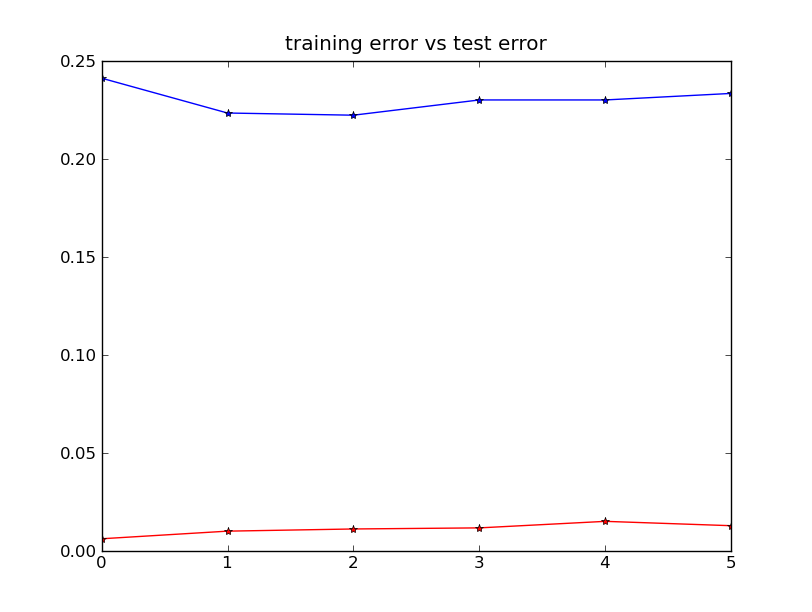
\includegraphics[width=4.5in]{WU5/trainingvstestD3R.png}
  \caption{Training error and test error vs stacking layers.}
  \label{figures:f1}
\end{figure}

\newpage

\begin{figure}[!ht]
  \centering
  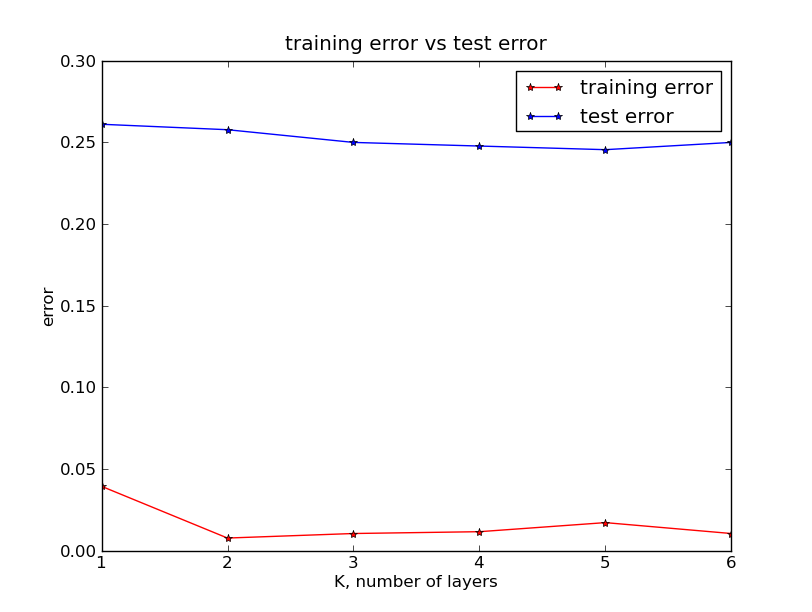
\includegraphics[width=4.5in]{WU5/trainingvstestD2R.png}
  \caption{Training error and test error vs stacking layers.}
  \label{figures:f2}
\end{figure}

\begin{figure}[!ht]
  \centering
  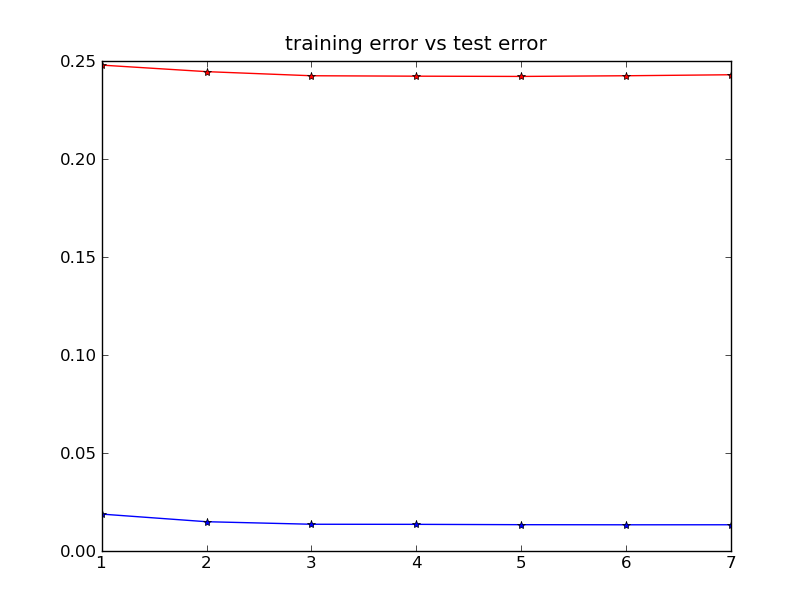
\includegraphics[width=4.5in]{WU5/CrossValidation.png}
  \caption{Cross validation training error and test error vs stacking layers.}
  \label{figures:f3}
\end{figure}

\newpage

Our stacking approaches consistently yielded just a few percentage points of
increased accuracy on the Cora dataset as opposed to the accuracy without any stacking. 
Comparing our results with those in previous work with Cora data \footnotemark[\value{footnote}]
we found similar error rates with models not using stacking, but previous work found as much as
12\% increase in accuracy using stacking where we only gained as much as 2\%. It may be that the
feature values we used could be improved, that with further investigation bootstrapping might yield
much better results, or we might try increasing the collective degree of each stacking step by 
looking at neighbors of neighbors. Overall, stacking has the potential to yield useful information
that can improve classification, but we found that performance is highly dependent on how that data is represented and whether
the connections are preserved when the data is mined.

\end{document}
